\subsection{Usuarios}

De igual manera que en la creación de roles, el apartado para crear usuarios se encuentra dentro de \textbf{“Directorio”}.

\begin{figure}[H]
    \centering
    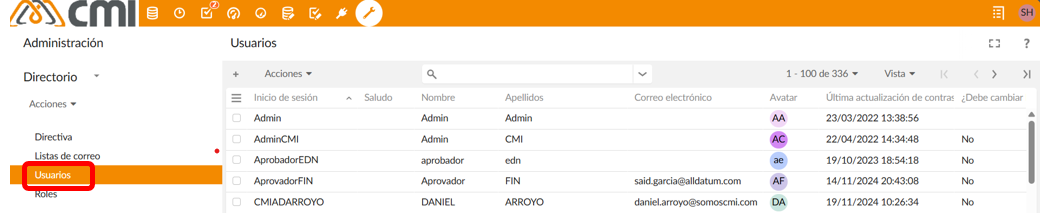
\includegraphics[width=0.8\textwidth]{RolesUsuario/ImgRolesUsuario/S01.png}
    \caption{Apartado de usuarios en Directorio}
\end{figure}

Para crear un nuevo usuario se dará clic en el símbolo de más (+).

\begin{figure}[H]
    \centering
    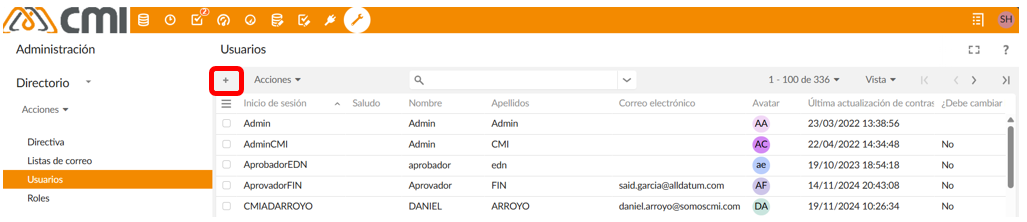
\includegraphics[width=0.8\textwidth]{RolesUsuario/ImgRolesUsuario/S02.png}
    \caption{Apartado de usuarios en Directorio}
\end{figure}